\documentclass[preprint,12pt]{elsarticle}
\usepackage[english]{babel}
\usepackage[utf8]{inputenc}
\usepackage{amsmath,amssymb,mathrsfs,mathtext,amsthm}
\usepackage{a4wide}
\usepackage[T2A]{fontenc}
\usepackage{subfig}
\usepackage{url}
\usepackage[usenames]{color}
\usepackage{colortbl}

\newcommand{\hdir}{.}
\usepackage{hyperref}       % clickable links
\usepackage{lineno}
\usepackage{graphicx,multicol}
\usepackage{epstopdf}
\usepackage{amsmath,amssymb,mathrsfs,mathtext}
\usepackage{tikz}
\usetikzlibrary{shapes,arrows,shadows}

\newtheorem{theorem}{Theorem}
\newtheorem{proposition}{Proposition}

\theoremstyle{definition}
\newtheorem{definition}{Definition}

\usepackage{algorithm}
\usepackage[noend]{algcompatible}

\usepackage{multirow}

\usepackage{caption}

%\renewcommand{\baselinestretch}{1.4}


\newcommand{\bx}{\mathbf{x}}
\newcommand{\by}{\mathbf{y}}
\newcommand{\bw}{\mathbf{w}}
\newcommand{\ba}{\mathbf{a}}
\newcommand{\bz}{\mathbf{z}}
\newcommand{\bb}{\mathbf{b}}
\newcommand{\bY}{\mathbf{Y}}
\newcommand{\bX}{\mathbf{X}}
\newcommand{\bu}{\mathbf{u}}
\newcommand{\bt}{\mathbf{t}}
\newcommand{\bp}{\mathbf{p}}
\newcommand{\bq}{\mathbf{q}}
\newcommand{\bc}{\mathbf{c}}
\newcommand{\bP}{\mathbf{P}}
\newcommand{\bT}{\mathbf{T}}
\newcommand{\bB}{\mathbf{B}}
\newcommand{\bQ}{\mathbf{Q}}
\newcommand{\bC}{\mathbf{C}}
\newcommand{\bE}{\mathbf{E}}
\newcommand{\bF}{\mathbf{F}}
\newcommand{\bU}{\mathbf{U}}
\newcommand{\bW}{\mathbf{W}}
\newcommand{\bbR}{\mathbb{R}}
\newcommand{\cA}{\mathcal{A}}
\newcommand{\T}{\mathsf{T}}
\newcommand{\bchi}{\boldsymbol{\chi}}
\newcommand{\bnu}{\boldsymbol{\nu}}
\newcommand{\bmu}{\boldsymbol{\mu}}
\newcommand{\btheta}{\boldsymbol{\theta}}
\newcommand{\bTheta}{\boldsymbol{\Theta}}
\newcommand{\bOne}{\boldsymbol{1}}
\newcommand{\bZero}{\boldsymbol{0}}
\newcommand{\argmin}{\mathop{\arg \min}\limits}
\newcommand{\argmax}{\mathop{\arg \max}\limits}

\begin{document}
	\begin{frontmatter}
		\title{Quadratic Programming Feature Selection for Multicorrelated Signal Decoding with Partial Least Squares\tnoteref{t1}}
		\tnotetext[t1]{The research was made possible by Government of the Russian Federation (Agreement 05.Y09.21.0018)}
		\author[mipt]{R.V.~Isachenko\corref{cor1}}
		\ead{roman.isachenko@phystech.edu}
		\author[ccas]{V.V.~Strijov}
		\ead{strijov@ccas.ru} 
		\cortext[cor1]{Corresponding author}
		
		\address[mipt]{
			Moscow Institute of Physics and Technology, 9 Institutskiy Per., Dolgoprudny, Moscow Region 141700, Russian Federation}
		\address[ccas]{A. A. Dorodnicyn Computing Centre, Federal Research Center “Computer Science and Control” of the Russian Academy of Sciences, 40 Vavilov Str., Moscow 119333, Russian Federation}
		
		\begin{abstract} 
			This paper is devoted to the dimensionality reduction problem in signal decoding.
			The challenge of this investigation is the redundancy in the data description. 
			High correlations among measurements lead to correlations in the input space. 
			This study considers the multivariate problem, and the target variable is a vector.
			In this case, the correlations occur in both the input and target spaces.
			Dimensionality reduction and feature selection are used to build simple and stable model.
			
			The partial least squares~(PLS) regression is used as the base model for the dimensionality reduction.
			The model projects the input and target data into the joint latent space and maximizes the covariances between the projections.
			To obtain the sparse model, the feature selection is applied.
			The majority of feature selection methods ignore the dependencies in the target space.
			The study suggests a novel approach to feature selection using a multivariate regression.
			The proposed approach extends the ideas of the quadratic programming feature selection~(QPFS) algorithm. 
			The QPFS algorithm selects the noncorrelated features that are relevant to the targets. 
			The proposed methods take into account the dependencies in the target space and select the features that are informative to all targets jointly.
			
			The computational experiment was carried out using the electrocorticogram (ECOG) dataset. 
			The proposed algorithms were compared using different criteria such as their stability and predictive performance.
			The algorithms give significantly better results compared to the baseline strategy.
			The QPFS approach was compared with the partial least squares~(PLS) regression.
			The best result is obtained by a combination of the QPFS and PLS algorithms.
			
		\end{abstract}
		\begin{keyword}
			partial least squares \sep quadratic programming feature selection \sep signal decoding
		\end{keyword}
	\end{frontmatter}

%%%%%%%%%%%%%%%%%%%%%%%%%%%%%%%%%%%%%%%%%%%%%%%%
\section{Introduction}
%%%%%%%%%%%%%%%%%%%%%%%%%%%%%%%%%%%%%%%%%%%%%%%%

The initial data in the fields of chemometrics~\cite{karimi2014leukemia,lin2016equivalence} and signal decoding~\cite{eliseyev2014stable,eliseyev2012l1} are high-dimensional and extremely redundant.
The models that are built on such data are instable. 
In addition, the redundant data description requires excessive computations, which lead to extended analisys times. 
To overcome this problem, dimensionality reduction~\cite{chun2010sparse,mehmood2012review} and feature selection~\cite{katrutsa2015stress,li2017feature} methods are used  for high-dimensional data modeling. 

The partial least squares~(PLS) is a widely used algorithm for dimensionality reduction~\cite{lauzon2018sequential,engel2017kernel,biancolillo2017extension,hervas2018sparse}. 
The PLS finds the optimal combinations of the initial features and uses these combinations as the model features. 
The algorithm projects the features and the targets onto the joint latent space and maximizes the covariances between the projected vectors. 
It allows researchers to save the information about the initial input and target matrices and find their relations. 
The dimensionality of the latent space is much less than the size of the initial data description. 
It leads to a stable linear model built on a small number of features. 
An overview of the advances in the PLS regression is given in~\cite{rosipal2006overview,rosipal2011nonlinear}.
For this model, we obtain the linear model with a small latent dimension.
However, the final model uses the whole range of the initial features, and it does not allow for the removal of useless features. 

Feature selection is a special case of dimensionality reduction when the latent representation is a subset of the initial data description. 
Here, the model is built on the subsets of the features. 
One of the approaches to feature selection is to maximize the feature relevances and minimize the pairwise feature redundancy. 
This approach was recently proposed and investigated in~\cite{ding2005minimum,yamada2014high}.
Quadratic programmic feature selection~(QPFS)~\cite{rodriguez2010quadratic} uses this approach to construct the optimization problem. It was shown in~\cite{katrutsa2017comprehensive} that the QPFS algorithm outperforms many existing feature selection methods for the univariate regression problem. 
The QPFS algorithm introduces two functions: $\text{Sim}$ and $\text{Rel}$.
$\text{Sim}$ estimates the redundancy between features, and $\text{Rel}$ contains the relevances between each feature and the target vector.
QPFS minimizes the Sim function and maximizes the Rel function simultaneously.
The algorithm solves the following optimization problem:
\begin{equation}
(1 - \alpha) \cdot \underbrace{\bz^{\T} \bQ \bz}_{\text{Sim}(\bX)} - \alpha \cdot \underbrace{ \bb^{\T} \bz}_{\text{Rel} (\bX, \bnu)} \rightarrow \min_{\substack{\bz \geq \bZero_n \\ \bOne_n^{\T} \bz=1}}.
\label{eq:qpfs_problem}
\end{equation}
Here, the columns of matrix~$\bX$ are the features, and~$\bnu$ is the target vector. 
The matrix~$\bQ \in \bbR^{n \times n}$ entries measure the pairwise similarities between features.
The vector $\bb \in \bbR^n$ expresses the similarities between each feature and the target vector.
The normalized vector~$\bz$ shows the importance of each feature.
Function~\eqref{eq:qpfs_problem} penalizes the dependent features using the Sim function and promotes the features that are relevant to the target using the Rel function.
The parameter~$\alpha$ controls the trade-off between Sim and Rel.
To measure the similarity, the authors of~\cite{rodriguez2010quadratic} use the absolute value of the sample correlation coefficient between pairs of features for the Sim function, and between the features and the target vector for the Rel function.

Paper~\cite{motrenko2018multi} proposes a multiway version of the QPFS algorithm for tensor ECoG-based data. 
It was shown that QPFS is an appropriate feature selection method for the signal decoding problem.
We consider the multivariate problem, where the dependent variable is a vector. 
It leads to correlations in the model targets. 
In this situation, feature selection algorithms do not take into account these dependencies.
Hence, the selected feature subset is not optimal in terms of its prediction.
We propose methods that take into account the dependencies in both the input and target spaces. 
It allows us to form a stable sparse model.
We refer to the original QPFS algorithm as our baseline for the computational experiment.

The main drawback of the QPFS algorithm is its computational costs. However, the original paper~\cite{rodriguez2010quadratic} suggests a way to solve the quadratic problem~\eqref{eq:qpfs_problem} efficiently. Additionally, in~\cite{prasad2013scaling}, the sequential minimal optimization framework is proposed for solving~\eqref{eq:qpfs_problem}.

The experiments were carried out using the ECoG dataset~\cite{shimoda2012decoding}.
We compared the proposed methods for multivariate feature selection with the baseline strategy and the PLS algorithm. 
The stability of the proposed methods was investigated by measuring how the feature selection solution changes with data bootstrapping.
The proposed algorithms outperform the baseline algorithm given the same number of features. 
The combination of the feature selection procedure and the PLS algorithm gives the best performance.

The main contributions of this paper are as follows:
\begin{itemize}
	\item addressing the dimensionality reduction problem for high-dimensional data,
	\item proposing new feature selection methods for multivariate regression with the analysis of the input and target spaces structures,
	\item comparing the proposed methods using a real ECoG dataset, and showing that the proposed methods give better feature subsets than the baseline method.
\end{itemize}


\section{Multivariate regression}

The goal is to forecast a dependent variable $\by \in \bbR^r$ with $r$ targets from an independent input object $\bx \in \bbR^n$ with $n$ features.
We assume that there is a linear dependence between the object $\bx$ and the target variable $\by$ as
\begin{equation}
\by = \bTheta \bx+ \boldsymbol{\varepsilon},
\label{eq:model}
\end{equation}
where $\bTheta \in \bbR^{r \times n}$ is the matrix of the model parameters, and $\boldsymbol{\varepsilon} \in \bbR^{r}$ is a residual vector.
One has to find the matrix of the model parameters~$\bTheta$ given a dataset $\left( \bX, \bY \right)$, where $\bX \in \bbR^{m \times n}$ is a design matrix and $\bY \in \bbR^{m \times r}$ is a target matrix:
\begin{equation*}
\bX = [\bx_1, \dots, \bx_m]^{\T} =  [\bchi_1, \dots, \bchi_n]; \quad \bY = [\by_1, \dots, \by_m]^{\T} =  [\bnu_1, \dots, \bnu_r].
\end{equation*}
The columns~$\bchi_j$ of~$\bX$ correspond to the object features, and the columns~$\bnu_j$ of~$\bY$ correspond to the targets.

The optimal parameters are determined by the minimization of an error function.
We define the quadratic loss function as follows:
\begin{equation}
\mathcal{L}(\bTheta | \bX, \bY) = {\left\| \underset{m \times r}{\mathbf{Y}}  - \underset{m \times n}{\bX} \cdot \underset{r \times n}{\bTheta}^{\T} \right\| }_2^2 \rightarrow\min_{\bTheta}.
\label{eq:loss_function}
\end{equation}
The solution of~\eqref{eq:loss_function} is given by
\begin{equation*}
\bTheta = \bY^{\T} \bX (\bX^{\T} \bX)^{-1}.
\end{equation*}

The linear dependent columns of~$\bX$ lead to an instable solution for the optimization problem~\eqref{eq:loss_function}.
If there is a vector $\boldsymbol{\alpha} \neq \bZero_n$ such that $\bX \boldsymbol{\alpha}= \bZero_m$, then adding~$\boldsymbol{\alpha}$ to any column of~$\bTheta$ does not change the value of the loss function $\mathcal{L}(\bTheta | \bX, \bY)$.
In this case, the matrix~$\bX^{\T} \bX$ is close to singular and is not invertible.
To avoid strong linear dependence, dimensionality reduction and feature selection are used.

%%%%%%%%%%%%%%%%%%%%%%%%%%%%%%%%%%%%%%%%%%%%%%%%
\section{Feature selection}
%%%%%%%%%%%%%%%%%%%%%%%%%%%%%%%%%%%%%%%%%%%%%%%%

The feature selection goal is to find the boolean vector~$\ba = \{0, 1\}^n$ in which the components indicate whether the feature is selected. 
To obtain the optimal vector~$\ba$ among all possible $2^n - 1$ options, we introduce the feature selection error function $S(\ba | \bX, \bY)$. 
We state the feature selection problem as follows:
\begin{equation}
\ba = \argmin_{\ba' \in \{0, 1\}^n} S(\ba' | \bX, \bY).
\label{eq:feature_selection}
\end{equation}
The goal of feature selection is to construct the appropriate function~$S(\ba | \bX, \bY)$. The particular examples for the considered feature selection algorithms are given below and summarized in Table~\ref{tbl:summary}.

Problem~\eqref{eq:feature_selection} is hard to solve due to the discrete binary domain~$\{0, 1\}^n$. We relax problem~\eqref{eq:feature_selection} to the continuous domain~$[0, 1]^n$. The relaxed feature selection problem is
\begin{equation}
\bz = \argmin_{\bz' \in [0, 1]^n} S(\bz' | \bX, \bY).
\label{eq:relaxed_feature_selection}
\end{equation}
Here, the vector~$\bz$ entries are the normalized feature importances.
First, we solve problem~\eqref{eq:relaxed_feature_selection} to obtain the feature importances~$\bz$. 
Then, the solution of~\eqref{eq:feature_selection} is recovered by thresholding as follows:
\begin{equation*}
\ba = [a_j]_{j=1}^n, \quad 
a_j = \begin{cases}
1, & z_j > \tau; \\
0, & \text{otherwise}.
\end{cases}
\end{equation*}
$\tau$ is a hyperparameter that is defined manually or chosen by cross-validation. 

Once the solution~$\ba$ of~\eqref{eq:feature_selection} is known, problem~\eqref{eq:loss_function} becomes
\begin{equation*}
\mathcal{L}(\bTheta_{\ba} | \bX_{\ba}, \bY) = {\left\| \mathbf{Y} - \bX_{\ba}\bTheta^{\T}_{\ba} \right\| }_2^2 \rightarrow\min_{\bTheta_{\ba}},
\end{equation*}
where subscript~$\ba$ indicates the sub matrix with the columns in which the components of~$\ba$ equal 1.

\subsection{Quadratic Programming Feature Selection}

Paper~\cite{katrutsa2017comprehensive} shows that QPFS outperforms many existing feature selection algorithms using different quality criteria.
The QPFS algorithm selects the noncorrelated features that are relevant to the target vector~$\bnu$ for the linear regression problem where~$r=1$ as follows:
\begin{equation*}
\| \bnu - \bX \btheta\|_2^2 \rightarrow\min_{\btheta \in \bbR^{n}}.
\end{equation*}

The authors of the original QPFS paper~\cite{rodriguez2010quadratic} suggested the following way to select~$\alpha$ for~\eqref{eq:qpfs_problem} and make $\text{Sim}(\bX)$ and $\text{Rel}(\bX, \bnu)$ have the same impacts:
\begin{equation*}
\alpha = \frac{\overline{\bQ}}{\overline{\bQ} + \overline{\bb}}, \quad \overline{\bQ} = \text{mean} (\bQ), \,\,\, \overline{\bb}= \text{mean} (\bb).
\end{equation*}
The QPFS parameters are defined as follows:
\begin{equation}
\bQ = \left[|\text{corr}(\bchi_i, \bchi_j)|\right]_{i,j=1}^n, \quad \bb = \left[|\text{corr}(\bchi_i, \bnu)|\right]_{i=1}^n.
\label{eq:qpfs_1d_qb}
\end{equation}
Here~$\text{corr}(\cdot, \cdot)$, is the absolute value of the sample Pearson correlation coefficient:
\begin{equation*}
\text{corr}(\bchi, \bnu) = \frac{\sum_{i=1}^m(\bchi_i - \overline{\bchi})( \bnu_i - \overline{\bnu})}{\sqrt{\sum_{i=1}^m(\bchi_i - \overline{\bchi})^2\sum_{i=1}^m(\bnu_i - \overline{\bnu})^2}}.
\end{equation*}
Other ways to define $\bQ$ and $\bb$ are considered in~\cite{katrutsa2017comprehensive}.

Problem~\eqref{eq:qpfs_problem} is convex if the matrix~$\bQ$ is positive semidefinite. In general, this is not always true.
To satisfy this condition, the matrix~$\bQ$ spectrum is shifted and matrix~$\bQ$ is replaced by $\bQ - \lambda_{\text{min}} \mathbf{I}$, where $\lambda_{\text{min}} $ is the minimum eigenvalue of~$\bQ$.

\subsection{Multivariate QPFS}

Here, we propose the algorithms for feature selection in the multivariate case. 
If the target space is multidimensional, it is prone to redundancy and correlations between the targets. 
In this section, we propose the algorithms that take into account the dependencies in both the input and target spaces.

\paragraph{Relevance aggregation (RelAgg)}

In~\cite{motrenko2018multi}, in order to apply the QPFS algorithm to the multivariate case ($r > 1$), feature relevances are aggregated through all $r$ components. The term $\text{Sim}(\bX)$ is still the same, and matrix~$\bQ$ is defined by~\eqref{eq:qpfs_1d_qb}. The vector $\bb$ is aggregated across all targets and is defined as
\begin{equation*}
\bb = \left[\sum_{k=1}^r|\text{corr}(\bchi_i, \bnu_k)|\right]_{i=1}^n.
\end{equation*}
The drawback of this approach is its insensitivity to the dependencies in the columns of~$\bY$. Observe the following example:
\begin{equation*}
\bX = [\bchi_1, \bchi_2, \bchi_3], \quad \bY = [\underbrace{\bnu_1, \bnu_1, \dots, \bnu_1}_{r-1}, \bnu_2].
\end{equation*}
We have 3 features and $r$ targets, where the first $r-1$ targets are identical.
The pairwise features similarities are given by matrix~$\bQ$.
Matrix $\bB$ entries five the pairwise features relevances to the targets.
Vector $\bb$ is obtained by the summation of matrix~$\bB$ over the columns
\begin{equation}
\bQ = \begin{bmatrix} 1 & 0 & 0\\ 0 & 1 & 0.8 \\ 0 & 0.8 & 1 \end{bmatrix}, \quad
\bB = \begin{bmatrix} 0.4 & \dots & 0.4 & 0 \\ 0.5 & \dots & 0.5 & 0.8 \\ 0.8 & \dots & 0.8 & 0.1 \end{bmatrix}, \quad
\bb = \begin{bmatrix} (r-1) \cdot 0.4 + 0 \\ (r-1) \cdot 0.5 + 0.8 \\ (r-1) \cdot 0.8 + 0.1 \end{bmatrix}.
\label{eq:qpfs_example}
\end{equation}
\vspace{0.5cm} \\
We would like to select only two features.
For such a configuration, the best feature subset is~$[\bchi_1, \bchi_2]$.
Feature~$\bchi_2$ predicts the second target~$\bnu_2$ and the combination of features~$\bchi_1, \bchi_2$ predicts the first component.
The QPFS algorithm for~$r=2$ gives the solution~$\bz = [0.37,	0.61,	0.02]$. It coincides with our knowledge.
However, if we add the collinear columns to matrix~$\bY$ and increase~$r$ to 5, the QPFS solution will be~$\bz = [0.40,	0.17, 0.43]$.
Here, we lose the relevant feature~$\bchi_2$ and select the redundant feature~$\bchi_3$.
The following subsections propose extensions to the QPFS algorithm that overcome the challenge of this example.

\paragraph{Symmetric importances (SymImp)}

To take into account the dependencies in the columns of matrix $\bY$, we extend the QPFS function~\eqref{eq:qpfs_problem} to the multivariate case.
We add the term~$\text{Sim}(\bY)$ and modify the term $\text{Rel}(\bX, \bY)$ as follows:
\begin{equation}
\alpha_1 \cdot \underbrace{\bz_x^{\T} \bQ_x \bz_x}_{\text{Sim}(\bX)} - \alpha_2 \cdot \underbrace{\bz_x^{\T} \bB \bz_y}_{\text{Rel}(\bX, \bY)} + \alpha_3 \cdot \underbrace{\bz_y^{\T} \bQ_y \bz_y}_{\text{Sim}(\bY)} \rightarrow \min_{\substack{\bz_x \geq \bZero_n, \, \bOne_n^{\T}\bz_x=1 \\ \bz_y \geq \bZero_r, \, \bOne_r^{\T}\bz_y=1}}.
\label{eq:symimp}
\end{equation}
We determine the entries of matrices $\bQ_x \in \bbR^{n \times n}$, $\bQ_y \in \bbR^{r \times r}$, and $\bB \in \bbR^{n \times r}$ in the following way:
\begin{equation*}
\bQ_x = \left[ |\text{corr}(\bchi_i, \bchi_j)| \right]_{i,j=1}^n, \quad
\bQ_y = \left[ |\text{corr}(\bnu_i, \bnu_j)| \right]_{i,j=1}^r, \quad
\bB =  \left[ |\text{corr}(\bchi_i, \bnu_j)| \right]_{\substack{i=1, \dots, n \\ j=1, \dots, r}}.
\end{equation*}
Vector~$\bz_x$ shows the features' importances, while $\bz_y$ is a vector of the targets importances.
The correlated targets will be penalized by $\text{Sim} (\bY)$ and have lower importances.

The coefficients $\alpha_1$, $\alpha_2$, and $\alpha_3$ control the influence of each term on function~\eqref{eq:symimp} and satisfy the following conditions:
\begin{equation*}
\alpha_1 + \alpha_2 + \alpha_3 = 1, \quad \alpha_i \geq 0, \, i = 1, 2, 3.
\end{equation*}
\begin{proposition}
	The balance between the terms~$\text{Sim}(\bX)$, $\text{Rel}(\bX, \bY)$, and $\text{Sim}(\bY)$ for the problem~\eqref{eq:symimp} is achieved by the following coefficients:
	\begin{equation}
	\alpha_1 \propto \overline{\bQ}_y \overline{\bB} ; \quad
	\alpha_2 \propto \overline{\bQ}_x \overline{\bQ}_y; \quad
	\alpha_3  \propto \overline{\bQ}_x \overline{\bB}.
	\label{eq:alpha_3}
	\end{equation}
	
\end{proposition}
\begin{proof}
	The desired values of $\alpha_1$, $\alpha_2$, and $\alpha_3$ are given by solving of the following equations:
	\begin{align*}
	&\alpha_1 + \alpha_2 + \alpha_3 = 1; \\
	&\alpha_1 \overline{\bQ}_x = \alpha_2 \overline{\bB} = \alpha_3 \overline{\bQ}_y.
	\end{align*}
	Here, the mean values~$\overline{\bQ}_x$, $\overline{\bB}$, and $\overline{\bQ}_y$ of the corresponding matrices~$\bQ_x$, $\bB$, and $\bQ_y$ are the mean values of the terms~$\text{Sim}(\bX)$, $\text{Rel}(\bX, \bY)$, and $\text{Sim}(\bY)$.
\end{proof}
To investigate the impact of~$\text{Sim}(\bY)$ on function~\eqref{eq:symimp}, we balance the terms $\text{Sim}(\bX)$ and $\text{Rel}(\bX, \bY)$ by fixing the proportion between~$\alpha_1$ and $\alpha_2$:
\begin{equation}
\alpha_1 = \frac{(1 - \alpha_3)\overline{\bB}}{\overline{\bQ}_x + \overline{\bB}}; \quad
\alpha_2 = \frac{(1 - \alpha_3)\overline{\bQ}_x}{\overline{\bQ}_x + \overline{\bB}}; \quad
\alpha_3 \in [0, 1].
\label{eq:alphas3}
\end{equation}

We apply the proposed algorithm to the discussed example~\eqref{eq:qpfs_example}.
The given matrix~$\bQ$ corresponds to matrix~$\bQ_x$.
We additionally define matrix~$\bQ_y$ by setting $\text{corr}(\bnu_1, \bnu_2) = 0.2$ and all others entries to one.
Figure~\ref{fig:features_vs_alpha} shows the importances of features~$\bz_x$ and targets~$\bz_y$ with respect to~$\alpha_3$.
If~$\alpha_3$ is small, the impacts of all targets are almost identical and feature~$\bchi_3$ dominates feature~$\bchi_2$. When~$\alpha_3$ becomes larger than~$0.2$, the importance~$\bz_{y,5}$ of target~$\bnu_5$ increases along with the importance of feature~$\bchi_2$.

\begin{figure}
	\centering
	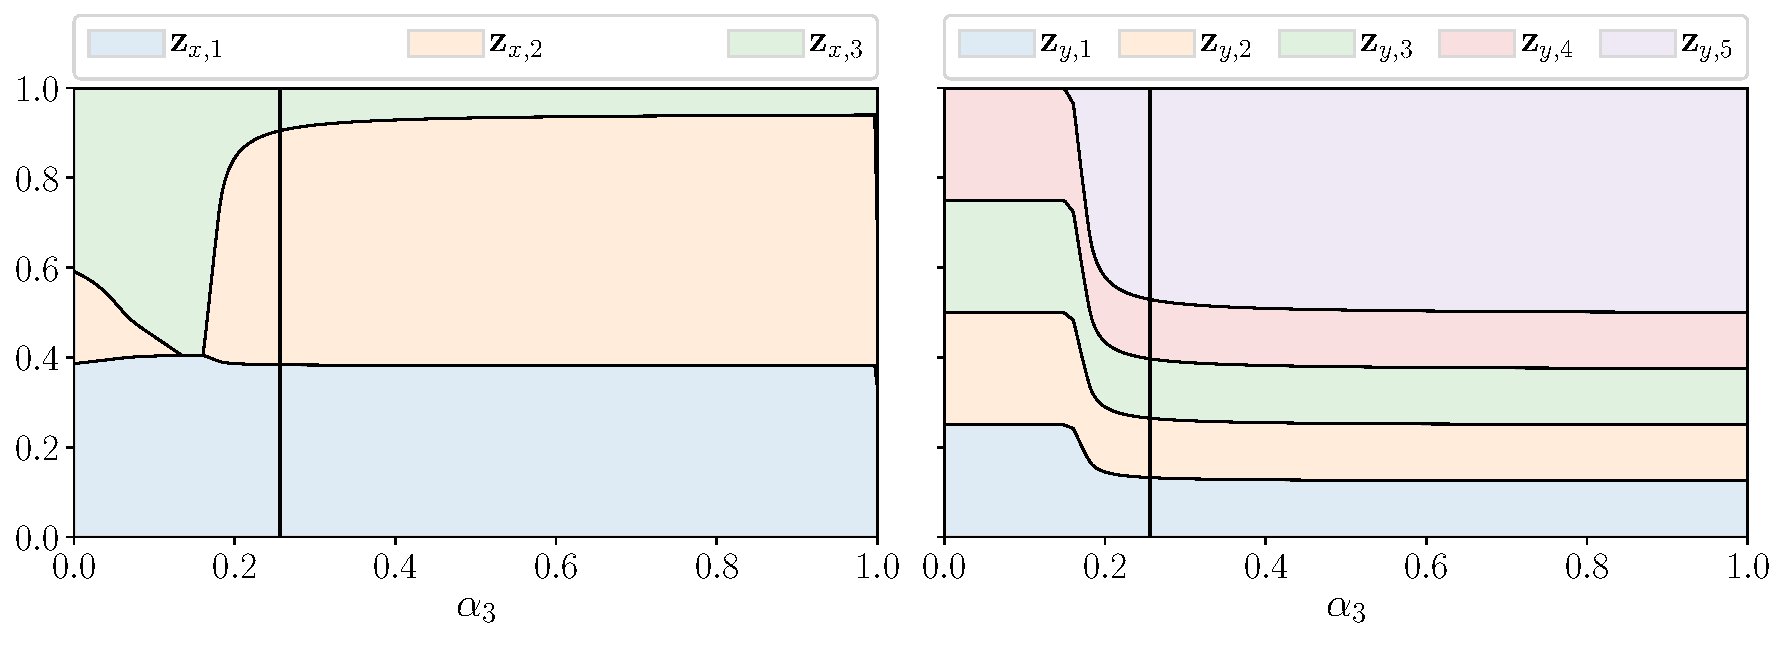
\includegraphics[width=\linewidth]{figs/features_vs_alpha.pdf}
	\caption{Feature importances $\bz_x$ and $\bz_y$ with respect to~$\alpha_3$ for the considered example}
	\label{fig:features_vs_alpha}
\end{figure}

\paragraph{Minimax QPFS (MinMax)}
Function~\eqref{eq:symimp} is symmetric with respect to~$\bz_x$ and $\bz_y$.
It penalizes the features that are correlated and irrelevant to the targets.
In addition, it penalizes the targets that are correlated and are not sufficiently explained by the features.
It leads to small importances for the targets that are weakly correlated with the features and large importances for the targets that are strongly correlated with the features.
This result contradicts the intuition.
Our goal is to predict all targets, especially those that are difficult to explain, using the selected relevant and noncorrelated features. We express this as two related problems:
\begin{align}
\alpha_1 \cdot \underbrace{\bz_x^{\T} \bQ_x \bz_x}_{\text{Sim}(\bX)} - \alpha_2 \cdot \underbrace{ \bz_x^{\T}\mathbf{B} \bz_y}_{\text{Rel}(\bX, \bY)} \rightarrow \min_{\substack{\bz_x \geq \bZero_n, \\ \bOne_n^{\T}\bz_x=1}};
\label{eq:x_qpfs}\\
\alpha_3 \cdot \underbrace{\bz_y^{\T} \bQ_y \bz_y}_{\text{Sim}(\bY)} + \alpha_2 \cdot \underbrace{ \bz_x^{\T} \mathbf{B} \bz_y}_{\text{Rel}(\bX, \bY)} \rightarrow \min_{\substack{\bz_y \geq \bZero_r,  \\ \bOne_r^{\T}\bz_y=1}}.
\label{eq:y_qpfs}
\end{align}
The difference between~\eqref{eq:x_qpfs} and~\eqref{eq:y_qpfs} is the sign of Rel.
In the input space, the nonrelevant components should have smaller importances.
Meanwhile, the targets that are not relevant to the features should have larger importances.
Problems~\eqref{eq:x_qpfs} and \eqref{eq:y_qpfs} are merged into the joint min-max or max-min formulation
\begin{equation}
\min_{\substack{\bz_x \geq \bZero_n \\ \bOne_n^{\T}\bz_x=1}} 	\max_{\substack{\bz_y \geq \bZero_r \\ \bOne_r^{\T}\bz_y=1}} f(\bz_x, \bz_y), \quad \left(\text {or} \, \max_{\substack{\bz_y \geq \bZero_r \\ \bOne_r^{\T}\bz_y=1}} \min_{\substack{\bz_x \geq \bZero_n \\ \bOne_n^{\T}\bz_x=1}} f(\bz_x, \bz_y)\right),
\label{eq:minmax}
\end{equation}
where
\begin{equation*}
f(\bz_x, \bz_y) = \alpha_1 \cdot \underbrace{\bz_x^{\T} \bQ_x \bz_x}_{\text{Sim}(\bX)} - \alpha_2 \cdot \underbrace{\bz_x^{\T} \bB \bz_y}_{\text{Rel}(\bX, \bY)} - \alpha_3 \cdot \underbrace{\bz_y^{\T} \bQ_y \bz_y}_{\text{Sim}(\bY)}.
\end{equation*}
\begin{theorem}
	For positive definite matrices $\bQ_x$ and $\bQ_y$, the max-min and min-max problems~\eqref{eq:minmax} have the same optimal value.
\end{theorem}
\begin{proof}
	We denote the following:
	\begin{equation*}
	\mathbb{C}^n = \{\bz : \bz \geq \bZero_n, \, \bOne_n^{\T}\bz=1\}, \quad \mathbb{C}^r = \{\bz : \bz \geq \bZero_r, \, \bOne_r^{\T}\bz=1\}.
	\end{equation*}
	The sets $\mathbb{C}^n$ and $\mathbb{C}^r$ are compact and convex. The function $f: \mathbb{C}^n \times \mathbb{C}^r \rightarrow \bbR$ is a continuous function. If $\bQ_x$ and $\bQ_y$ are positive definite matrices, function~$f$ is convex-concave. I.e.,
	$f(\cdot, \bz_y): \mathbb{C}^n \rightarrow \bbR$ is convex for a fixed~$\bz_y$, and $f(\bz_x, \cdot): \mathbb{C}^r \rightarrow \bbR$ is concave for a fixed~$\bz_x$.
	In this case, Neumann's minimax theorem states that
	\begin{equation*}
	\min_{\bz_x \in \mathbb{C}^n} \max_{\bz_y \in \mathbb{C}^r} f(\bz_x, \bz_y) = \max_{\bz_y \in \mathbb{C}^r} \min_{\bz_x\in \mathbb{C}^n} f(\bz_x, \bz_y).
	\end{equation*}
\end{proof}

To solve the min-max problem~\eqref{eq:minmax}, we fix some~$\bz_x \in \mathbb{C}^n$. For a fixed vector~$\bz_x$, we solve the problem
\begin{equation}
\max_{\bz_y \in \mathbb{C}_r} f(\bz_x, \bz_y) = \max_{\substack{\bz_y \geq \bZero_r \\ \bOne_r^{\T}\bz_y=1}} \bigl[\alpha_1 \cdot \bz_x^{\T} \bQ_x \bz_x - \alpha_2 \cdot \bz_x^{\T} \bB \bz_y - \alpha_3 \cdot \bz_y^{\T} \bQ_y \bz_y \bigr].
\label{eq:fixed_ax}
\end{equation}
The Lagrangian for this problem is
\begin{equation*}
L(\bz_x, \bz_y, \lambda, \bmu) = \alpha_1 \cdot \bz_x^{\T} \bQ_x \bz_x - \alpha_2 \cdot \bz_x^{\T} \bB \bz_y - \alpha_3 \cdot \bz_y^{\T} \bQ_y \bz_y + \lambda \cdot  (\bOne_r^{\T} \bz_y - 1) + \bmu^{\T} \bz_y.
\end{equation*}
Here, the Lagrange multipliers $\bmu$ that correspond to the inequality constraints $\bz_y \geq \bZero_r$ are restricted to being nonnegative.
The dual problem is
\begin{equation}
\min_{\lambda, \, \bmu \geq \bZero_r} g(\bz_x, \lambda, \bmu) = \min_{\lambda, \, \bmu \geq \bZero_r}  \left[\max_{\bz_y \in \bbR^r} L(\bz_x, \bz_y, \lambda, \bmu) \right].
\label{eq:dual}
\end{equation}
The strong duality holds for quadratic problem~\eqref{eq:fixed_ax} with the positive definite matrices~$\bQ_x$ and~$\bQ_y$. Therefore, the optimal value for~\eqref{eq:fixed_ax} equals the optimal value for~\eqref{eq:dual}. It allows us to solve the problem
\begin{equation}
\min_{\bz_x \in \mathbb{C}^n, \, \lambda, \, \bmu \geq \bZero_r} g(\bz_y, \lambda, \bmu)
\label{eq:dual_maxmin}
\end{equation}
instead of~\eqref{eq:minmax}.

By setting the gradient of the Langrangian $\nabla_{\bz_y} L(\bz_x, \bz_y, \lambda, \bmu)$ equal to zero, we obtain an optimal value for~$\bz_y$:
\begin{equation}
\bz_y = \frac{1}{2\alpha_3} \bQ_y^{-1} \left( - \alpha_2 \cdot \bB^{\T} \bz_x +\lambda \cdot \bOne_r + \bmu \right).
\label{eq:ax}
\end{equation}
The dual function is equal to
\begin{multline}
g(\bz_x, \lambda, \bmu)
= \max_{\bz_y \in \bbR^r} L(\bz_x, \bz_y, \lambda, \bmu) =
\bz_x^{\T} \left( - \frac{\alpha_2^2}{4\alpha_3} \cdot \bB \bQ_y^{-1} \bB^{\T} - \alpha_1 \cdot \bQ_x\right) \bz_x \\ - \frac{1}{4 \alpha_3} \lambda^2 \cdot \bOne_r^{\T} \bQ_y^{-1} \bOne_r - \frac{1}{4 \alpha_3} \cdot \bmu^{\T} \bQ_y^{-1} \bmu + \frac{\alpha_2}{2 \alpha_3} \lambda \cdot \bOne_r^{\T} \bQ_y^{-1} \bB^{\T} \bz_x \\ - \frac{1}{2 \alpha_3} \lambda \cdot \bOne_r^{\T} \bQ_y^{-1} \bmu + \frac{\alpha_2}{2 \alpha_3} \cdot \bmu^{\T} \bQ_y^{-1} \bB^{\T} \bz_x + \lambda.
\label{eq:dual_quadratic_form}
\end{multline}
It represents the quadratic problem~\eqref{eq:dual_maxmin} with~$n + r + 1$ variables.

\paragraph{Asymmetric Importance (AsymImp)}
The natural way to overcome the problem of the SymImp strategy is to add penalties for targets that are correlated with features.
We add the term~$\bb^{\T} \bz_y$ to the term $\text{Rel}(\bX, \bY)$ as follows:
\begin{equation}
\alpha_1 \cdot \underbrace{\bz_x^{\T} \bQ_x \bz_x}_{\text{Sim}(\bX)} - \alpha_2 \cdot  \underbrace{\left(\bz_x^{\T} \bB \bz_y - \bb^{\T} \bz_y \right) }_{\text{Rel}(\bX, \bY)} + \alpha_3 \cdot \underbrace{\bz_y^{\T} \bQ_y \bz_y}_{\text{Sim}(\bY)} \rightarrow \min_{\substack{\bz_x \geq \bZero_n, \, \bOne_n^{\T}\bz_x=1 \\ \bz_y \geq \bZero_r, \, \bOne_r^{\T}\bz_y=1}}.
\label{eq:asymimp}
\end{equation}
\begin{proposition}
	Let vector $\bb$ equal
	\begin{equation*}
	b_j = \max_{i=1, \dots n} [\bB]_{i, j}.
	\end{equation*}
	Then, the importance coefficients for vector~$\bz_y$ will be nonnegative in~$\text{Rel}(\bX, \bY)$ for problem~\eqref{eq:asymimp}.
\end{proposition}
\begin{proof}
	The proposition follows from the fact that
	\[
	\sum_{i=1}^n  z_i b_{ij} \leq \left(\sum_{i=1}^n z_i \right)\max_{i=1, \dots n} b_{ij} = \max_{i=1, \dots n} b_{ij},
	\]
	where $z_i \geq 0$ and $\sum_{i=1}^nz_i = 1$.
\end{proof}
Hence, function~\eqref{eq:asymimp} encourages the features that are relevant to the targets and encourages the targets that are not sufficiently correlated with the features. 
\begin{proposition}
	The balance between the terms~$\text{Sim}(\bX)$, $\text{Rel}(\bX, \bY)$, and $\text{Rel}(\bX, \bY)$ for the problem~\eqref{eq:asymimp} is achieved by the following coefficients:
	\begin{equation*}
	\alpha_1 \propto \overline{\bQ}_y \left( \overline{\bb} - \overline{\bB}\right); \quad
	\alpha_2 \propto \overline{\bQ}_x \overline{\bQ}_y; \quad
	\alpha_3  \propto \overline{\bQ}_x \overline{\bB}.
	\end{equation*}
\end{proposition}
\begin{proof}
	The desired values of $\alpha_1$, $\alpha_2$, and $\alpha_3$ are given by the solutions to the following equations:
	\begin{align}
	&\alpha_1 + \alpha_2 + \alpha_3 = 1; \\
	&\alpha_1 \overline{\bQ}_x = \alpha_2 \overline{\bB}; \label{eq:asymimp_balance1}\\
	&\alpha_2 \left(\overline{\bb} - \overline{\bB} \right) = \alpha_3 \overline{\bQ}_y.
	\label{eq:asymimp_balance2}
	\end{align}
	Here, we balance $\text{Sim}(\bX)$ with the first term of~$\text{Rel}(\bX, \bY)$ using~\eqref{eq:asymimp_balance1} and $\text{Sim}(\bY)$ with the full~$\text{Rel}(\bX, \bY)$ using~\eqref{eq:asymimp_balance2}.
\end{proof}
\begin{proposition}
	For the case of $r=1$, the proposed functions~\eqref{eq:symimp},~\eqref{eq:minmax}, and~\eqref{eq:asymimp} coincide with the original QPFS algorithm~\eqref{eq:qpfs_problem}.
	
	\begin{proof}
		If $r$ is equal to 1, then $\bQ_y = q_y$ is a scalar, $\bz_y = 1$, and $\bB = \bb$. It reduces problems~\eqref{eq:symimp},~\eqref{eq:minmax}, and~\eqref{eq:asymimp} to
		\begin{equation*}
		\alpha_1 \cdot \bz_x^{\T} \bQ_x \bz_x - \alpha_2 \cdot \bz_x^{\T} \bb \rightarrow \min_{\bz_x \geq \bZero_n, \, \bOne_n^{\T}\bz_x=1} .
		\end{equation*}
		Setting $\alpha = \frac{\alpha_2}{\alpha_1 + \alpha_2}$ represents the original QPFS problem~\eqref{eq:qpfs_problem}.
	\end{proof}
\end{proposition}

Table~\ref{tbl:summary} shows the core ideas and error functions for each method and summarizes all the proposed strategies for multivariate feature selection. 
RelAgg is the baseline strategy, and it does not consider the target space correlations.
SymImp penalizes the pairwise target correlations.
MinMax are more sensitive to the targets that are difficult to predict.
The AsymImp strategy adds the term to the SymImp function to make the features and targets have asymmetric influences. 


\begin{table}
	\centering
	\caption{Overview of the proposed multivariate QPFS algorithms}
	\small{
		\begin{tabular}{c|c|c}
			\hline
			Algorithm & Idea & Error function $S(\bz | \bX, \bY)$ \\
			\hline && \\ [-.5em]
			RelAgg & $\min \bigl[ \text{Sim}(\bX) - \text{Rel}(\bX, \bY) \bigr] $ & $\min\limits_{\bz_x} \bigl[ (1 - \alpha) \cdot \bz_x^{\T} \bQ_x \bz_x - \alpha \cdot \bz_x^{\T} \bB \bOne_r \bigr] $ \\ &&\\[-.5em]
			SymImp & $\begin{aligned} \min \, \bigl[ \text{Sim}(\bX) & - \text{Rel}(\bX, \bY) \\ & + \text{Sim}(\bY) \bigr] \end{aligned}$ & $ \min\limits_{\bz_x, \, \bz_y} \left[ \alpha_1 \cdot \bz_x^{\T} \bQ_x \bz_x - \alpha_2 \cdot \bz_x^{\T} \bB \bz_y + \alpha_3 \cdot \bz_y^{\T} \bQ_y \bz_y \right] $\\ &&\\ [-.5em]
			MinMax & $\begin{aligned} &\min \, \bigl[ \text{Sim}(\bX) - \text{Rel}(\bX, \bY) \bigr]  \\ & \max \bigl[\text{Rel}(\bX, \bY) + \text{Sim}(\bY) \bigr] \end{aligned}$ & $	\min\limits_{\bz_x} 	\max\limits_{\bz_y} \bigl[\alpha_1 \cdot \bz_x^{\T} \bQ_x \bz_x - \alpha_2 \cdot \bz_x^{\T} \bB \bz_y - \alpha_3 \cdot \bz_y^{\T} \bQ_y \bz_y \bigr]$ \\ &&\\ [-.5em]
			AsymImp & $\begin{aligned} & \min \, \bigl[ \text{Sim}(\bX) - \text{Rel}(\bX, \bY) \bigr]\\ &  \max \bigl[\text{Rel}(\bX, \bY) + \text{Sim}(\bY) \bigr] \end{aligned}$ & $\min\limits_{\bz_x, \bz_y} \bigl[ \alpha_1 \cdot \bz_x^{\T} \bQ_x \bz_x - \alpha_2 \cdot \left(\bz_x^{\T} \bB \bz_y - \bb^{\T} \bz_y \right) + \alpha_3 \cdot \bz_y^{\T} \bQ_y \bz_y \bigr]$\\ 
			\hline
	\end{tabular}}
	\label{tbl:summary}
\end{table}


%%%%%%%%%%%%%%%%%%%%%%%%%%%%%%%%%%%%%%%%%%%%%%%%
\subsection{Dimensionality reduction}
%%%%%%%%%%%%%%%%%%%%%%%%%%%%%%%%%%%%%%%%%%%%%%%%

To eliminate the linear dependence and reduce the dimensionality of the input space, principal components analysis (PCA) is a widely used algorithm. 
The main disadvantage of the PCA method is that it is insensitive to the interrelation between the features and the targets.
The partial least squares algorithm projects the design matrix~$\bX$ and the target matrix~$\bY$ to the latent space with low dimensionality ($l < n$).
The PLS algorithm finds the latent space matrices $\bT, \bU \in \mathbb{R}^{m \times l}$ that best describe the original matrices~$\bX$ and~$\bY$.

The design matrix~$\bX$ and the target matrix~$\bY$ are projected into the latent space in the following way:
\begin{align}
\label{eq:PLS_X}
\underset{m \times n}{\bX} 
&= \underset{m \times l}{\bT} \cdot \underset{l \times n}{\bP^{\T}} + \underset{m \times n}{\bF} 
= \sum_{k=1}^l \underset{m \times 1}{\bt_k} \cdot \underset{1 \times n}{\bp_k^{\T}} + \underset{m \times n}{\bF},\\
\label{eq:PLS_Y}
\underset{m \times r}{\bY} 
&= \underset{m \times l}{\bU} \cdot \underset{l \times r}{\bQ^{\T}} + \underset{m \times r}{\bE}
=  \sum_{k=1}^l  \underset{m \times 1}{\bu_k} \cdot \underset{1 \times r}{\bq_k^{\T}} +  \underset{m \times r}{\bE},
\end{align}
where $\bT$ and $\bU$ are the scores matrices in the latent space, $\bP$ and $\bQ$ are the loading matrices, $\bE$ and $\bF$ are residual matrices. The PLS maximizes the linear relation between the columns of matrices~$\bT$ and~$\bU$ as
\begin{equation*}
\bU \approx \bT \bB, \quad \bB = \text{diag}(\beta_k), \quad \beta_k = \bu_k^{\T}\bt_k / (\bt_k^{\T}\bt_k).
\end{equation*}
We use the PLS algorithm as the dimensionality reduction algorithm in this research.

To obtain the model prediction and find the model parameters, we multiply both sides of~\eqref{eq:PLS_X} by~$\bW$. 
Since the residual matrix~$\bE$ rows are orthogonal to the columns of~$\bW$, we have
\begin{equation*}
\bX \bW = \bT \bP^{\T} \bW.
\end{equation*}
The linear transformation between objects in the input and latent spaces is the following
\begin{equation}
\bT = \bX \bW^*, \quad \text{where } \bW^* = \bW (\bP^{\T} \bW)^{-1}.
\label{eq:W*}
\end{equation}
The matrix of the model parameters~\eqref{eq:model} could be found from equations~\eqref{eq:PLS_Y} and~\eqref{eq:W*} as
\begin{equation}
\bY = \bU \bQ^{\T} + \bE \approx \bT \bB \bQ^{\T}+ \bE = \bX \bW^* \bB \bQ^{\T} + \bE = \bX \bTheta + \bE.
\label{eq:pls_model}
\end{equation}
Thus, the model parameters~\eqref{eq:model} are equal to
\begin{equation*}
\bTheta = \bW (\bP^{\T} \bW)^{-1} \bB \bQ^{\T}.
\end{equation*}

The final model~\eqref{eq:pls_model} is a linear model that are low-dimensional in the latent space. 
It reduces the data redundancy and increases the model stability. 

%%%%%%%%%%%%%%%%%%%%%%%%%%%%%%%%%%%%%%%%%%%%%%%%
\section{Experiment}
%%%%%%%%%%%%%%%%%%%%%%%%%%%%%%%%%%%%%%%%%%%%%%%%

To evaluate the selected feature subset, we introduce criteria that estimate the quality of feature selection.
We measure the smulticorrelation using the mean value of miltiple correlation coefficient as follows:
\begin{equation*}
R^2 = \frac{1}{r} \text{tr} \left( \bC^{\T} \mathbf{R}^{-1} \bC \right); \quad \text{where }\bC = [ \text{corr}(\bchi_i, \bnu_j)]_{\substack{i=1, \dots, n \\ j=1, \dots, r}}, \, \mathbf{R} = [ \text{corr}(\bchi_i, \bchi_j)]_{i, j = 1}^n.
\end{equation*}
This coefficient lies between 0 and 1. A bigger $R^2$ means that we have a better feature subset.

The model stability is given by the logarithmic ratio between the minimum eigenvalue~$\lambda_{\min}$ and maximum eigenvalue~$\lambda_{\max}$ of matrix~$\bX^{\T} \bX$:
\begin{equation*}
\text{Stability} = \ln \frac{\lambda_{\min}}{\lambda_{\max}}.
\end{equation*}
A smaller Stability value indicates less multicollinearity in matrix~$\bX$.

The scaled Root Mean Squared Error (sRMSE) shows the quality of the model prediction. We estimate the sRMSE using train and test data.
\begin{equation*}
\text{sRMSE}(\bY, \widehat{\bY}_{\ba}) = \sqrt{\frac{\text{MSE} (\bY, \widehat{\bY}_{\ba})}{\text{MSE} (\bY, \overline{\bY})}} =  \frac{\| \bY - \widehat{\bY}_{\ba} \|_2}{\| \bY - \overline{\bY} \|_2}.
\end{equation*}
Here, $\widehat{\bY}_{\ba} = \bX_{\ba} \bTheta_{\ba}^{\T}$ is the model prediction and $\overline{\bY}$ is the constant prediction obtained by averaging the targets across all objects.
The error on the test set should be as small as possible.

The Bayesian Information Criteria (BIC) incorporates a trade-off between the prediction quality and the size of selected subset~$\|\ba\|_0 = \#\{j: a_j \neq 0\}= \sum_{j=1}^n a_j$:
\begin{equation*}
\text{BIC} = m \ln \left( \text{MSE} ( \bY, \widehat{\bY}_{\ba})\right) + \| \ba \|_0 \cdot \ln m,
\end{equation*}
A smaller value of BIC means a better feature subset.

\subsection{Data}

We conducted a computational experiment with the ECoG data from the NeuroTycho project~\cite{shimoda2012decoding}.
The ECoG data consist of brain voltage signals recorded over 32 channels.
The goal is to predict 3D hand positions in subsequent moments given the input signal.
The initial voltage signals are transformed to the spatial-temporal representation using the wavelet transformation with the Morlet mother wavelet.
The procedure of extracting the feature representation from the raw data is described in detail in~\cite{chao2010long,eliseyev2016penalized}.
We unfold the data and feature description at each time moment has dimension of size 32 (channels) $\times$ 27 (frequencies) = 864.
Each object is the representation of the local historical time segment with duration $\Delta t = 1s$. The time step between objects is $\delta t =  0.05s$.
The final matrices are $\bX \in \bbR^{18900 \times 864}$ and $\bY \in \bbR^{18900 \times 3k}$, where $k$ is the number of timestamps that we predict.
We split our data into train and test parts with the ratio 0.67. 
Example of the initial brain signals and the corresponding hand trajectory is shown in Figure~\ref{fig:ecog_data}.

\begin{figure}
	\centering
	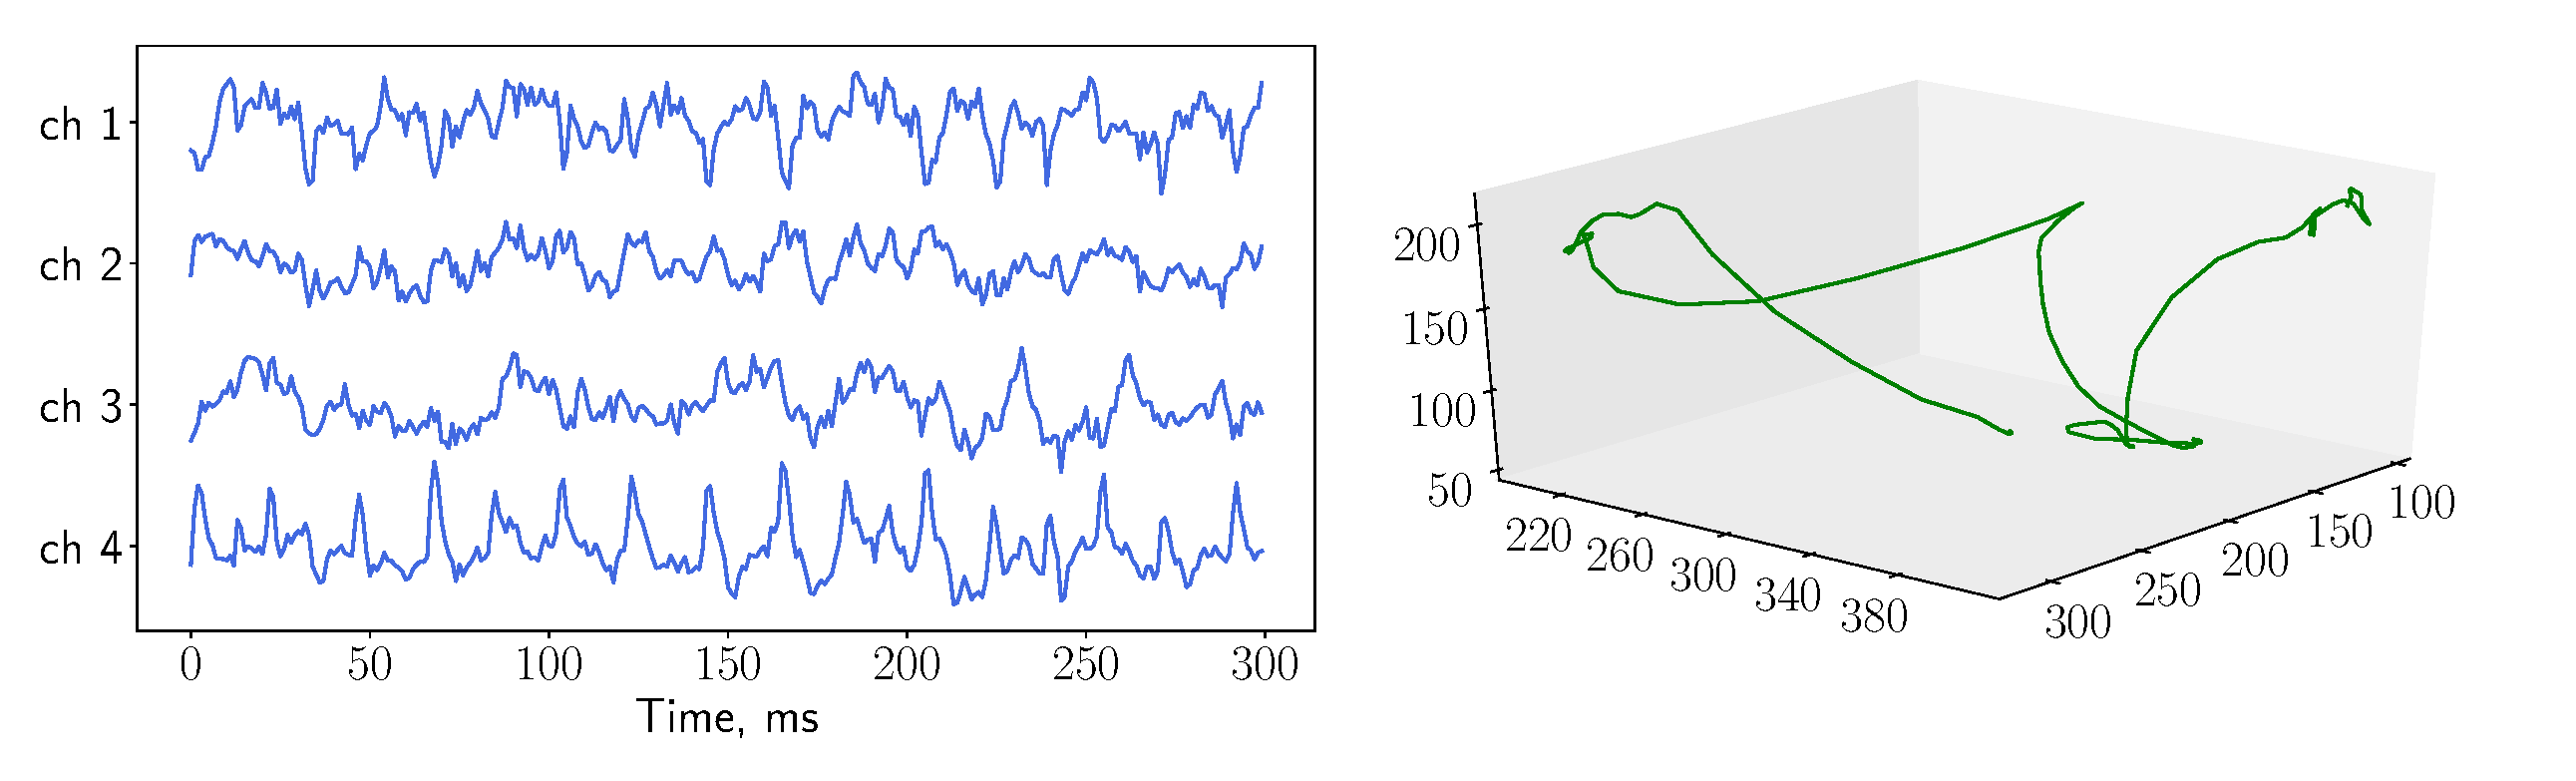
\includegraphics[width=\linewidth]{figs/ecog_data}
	\caption{Brain signals (left plot) and 3D hand coordinates (right plot)}
	\label{fig:ecog_data}
\end{figure}

%%%%%%%%%%%%%%%%%%%%%%%%%%%%%%%%%%%%%%%%%%%%%%%%
\subsection{Results}
%%%%%%%%%%%%%%%%%%%%%%%%%%%%%%%%%%%%%%%%%%%%%%%%

Figure~\ref{fig:corr_matrix} shows the dependencies in the matrices~$\bX$ and~$\bY$ for the ECoG data. The frequencies in the matrix~$\bX$ are highly correlated. 
In the target matrix~$\bY$, the correlations between axes are not significant in comparison with the correlations between consequent moments and these correlations decay with time.
\begin{figure}[h]
	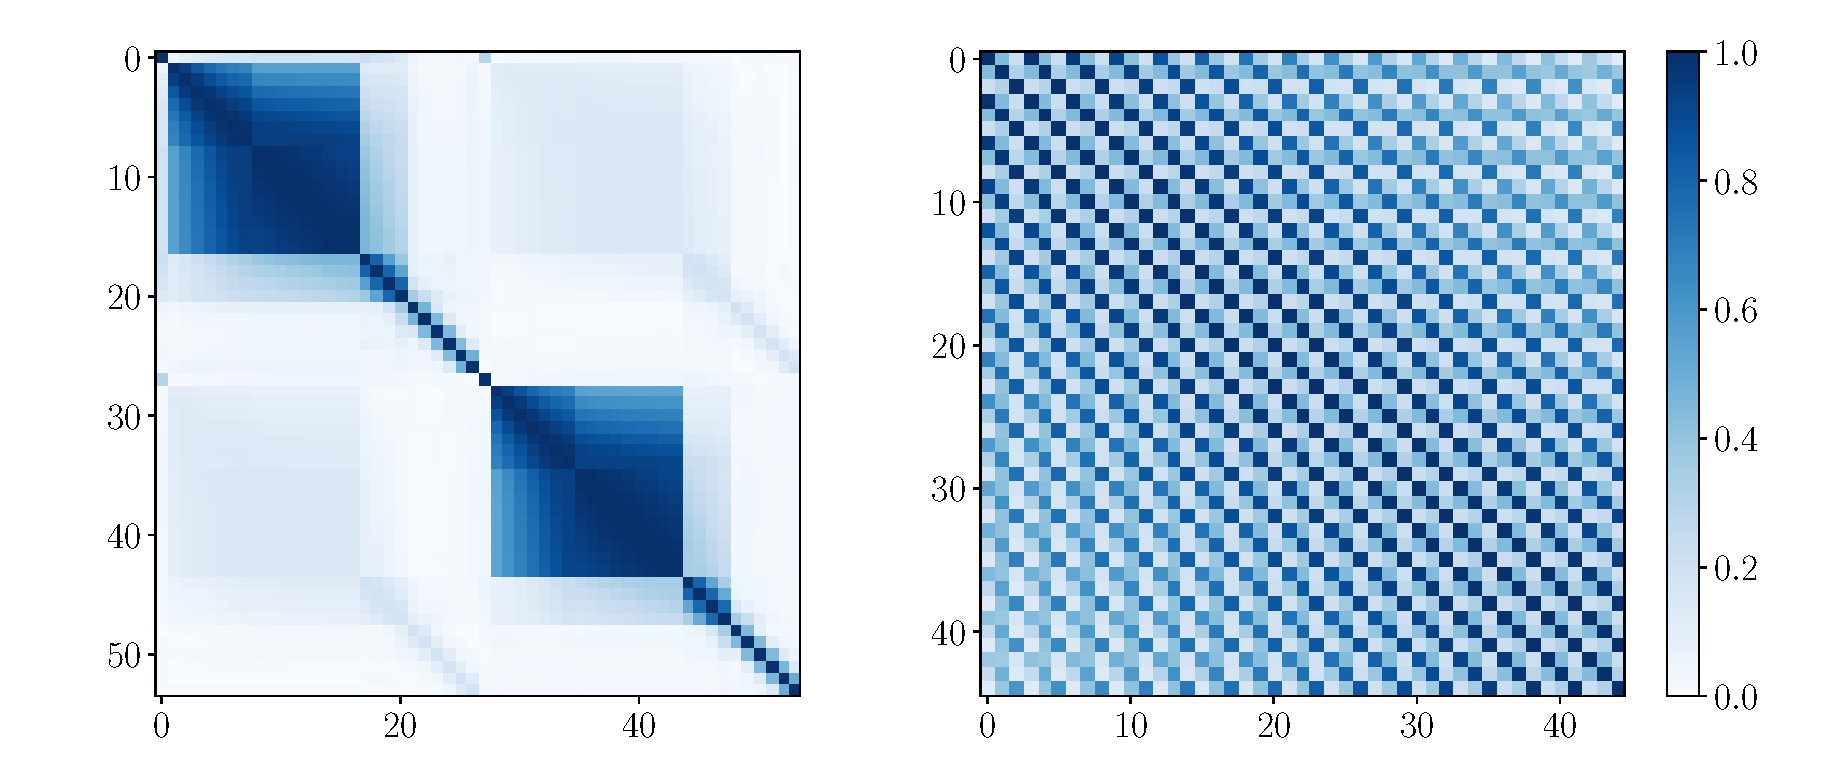
\includegraphics[width=\linewidth]{figs/corr_matrix.eps}
	\caption{Correlation matrices for $\bX$ and $\bY$}
	\label{fig:corr_matrix}
\end{figure}

We apply the QPFS algorithm with the SymImp strategy for different values of~$\alpha_3$ according to formula~\eqref{eq:alphas3}.
The dependencies between target importances~$\bz_y$ with respect to~$\alpha_3$ for different values of~$k$ are shown in Figure~\ref{fig:features_vs_alpha_ecog}.
The targets importances are almost the same for the predicted wrist coordinates with only one timestamp $k = 1$, 
which reflects the independence between the $x$, $y$, and $z$ coordinates.
For $k = 2$ and $k = 3$, the importances of some targets become zero when~$\alpha_3$ increases.
The vertical lines correspond to the optimal value of~$\alpha_3$ obtained by~\eqref{eq:alpha_3}. 
The target importances~$\bz_y$ for this value of~$\alpha_3$ are similar. 
Thus, the algorithm does not distinguish the targets for $k=1, 2, 3$.

\begin{figure}[h]
	\begin{minipage}{.5\linewidth}
		\subfloat{
			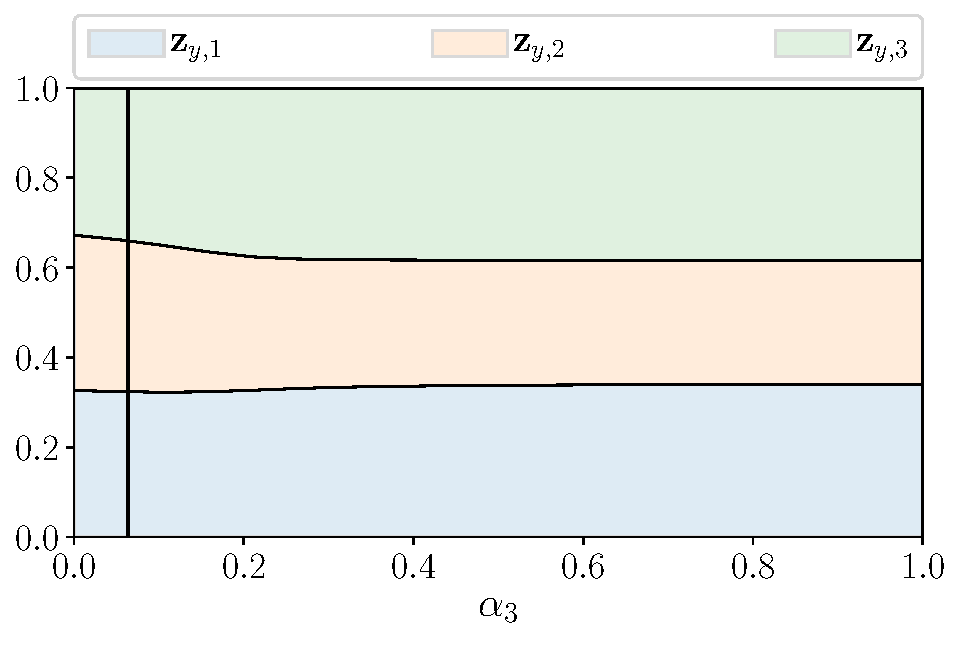
\includegraphics[width=\linewidth]{figs/features_vs_alpha_ecog_3.pdf}}
	\end{minipage}%
	\begin{minipage}{.5\linewidth}
		\subfloat{
			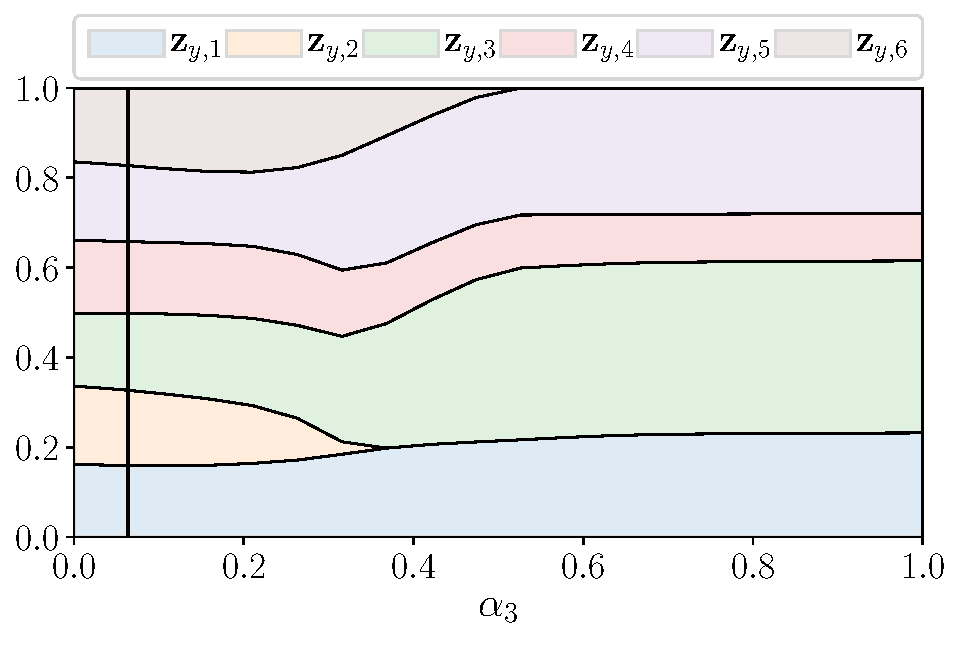
\includegraphics[width=\linewidth]{figs/features_vs_alpha_ecog_6.pdf}}
	\end{minipage}\par\medskip
	\subfloat{
		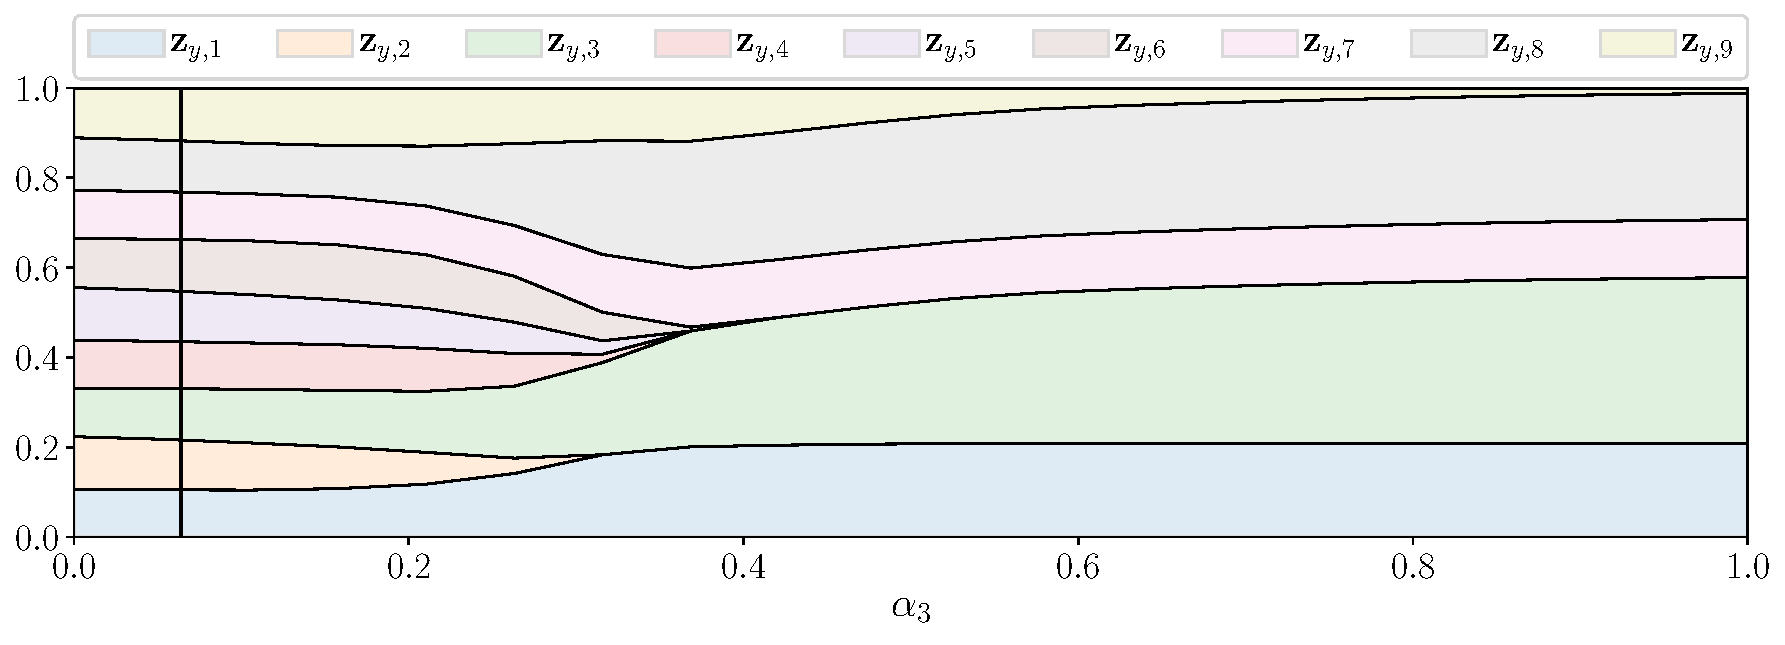
\includegraphics[width=\linewidth]{figs/features_vs_alpha_ecog_9.pdf}}
	
	\caption{Target importances~$\bz_y$ with respect to~$\alpha_3$ for QPFS with Symmetric Importance}
	\label{fig:features_vs_alpha_ecog}
\end{figure}

We compare the proposed strategies of the multivariate QPFS that are given in Table~\ref{tbl:summary} for the ECoG dataset. 
First, we apply all the methods to obtain the feature importances. 
Then, we fit a linear model with an increasing number of features. 
For each method, the features are sorted by their obtained importances. 
We show how the described quality criteria change with the increasing feature set size. 
Figure~\ref{fig:ecog_3_30_metrics} illustrates the results for the prediction of $k = 30$ timestamps. 
Here, the feature importance threshold $\tau$ is represented by colored ticks. 
These thresholds are larger for the proposed methods in comparison to the baseline RelAgg strategy. 
The SymImp strategy has the largest threshold, and it does not allow one to obtain a small feature subset.
However, this strategy shows the best performance in terms of the sRMSE using the test data.
The second performance is given by AsymImp.
All proposed algorithms give smaller test errors compared to the RelAgg strategy. 
The Stability criteria is also increased for the proposed algorithms.
Here, we consider the AsymImp strategy as the best in terms of the predictive quality and the size of selected feature subset.

\begin{figure}[h]
	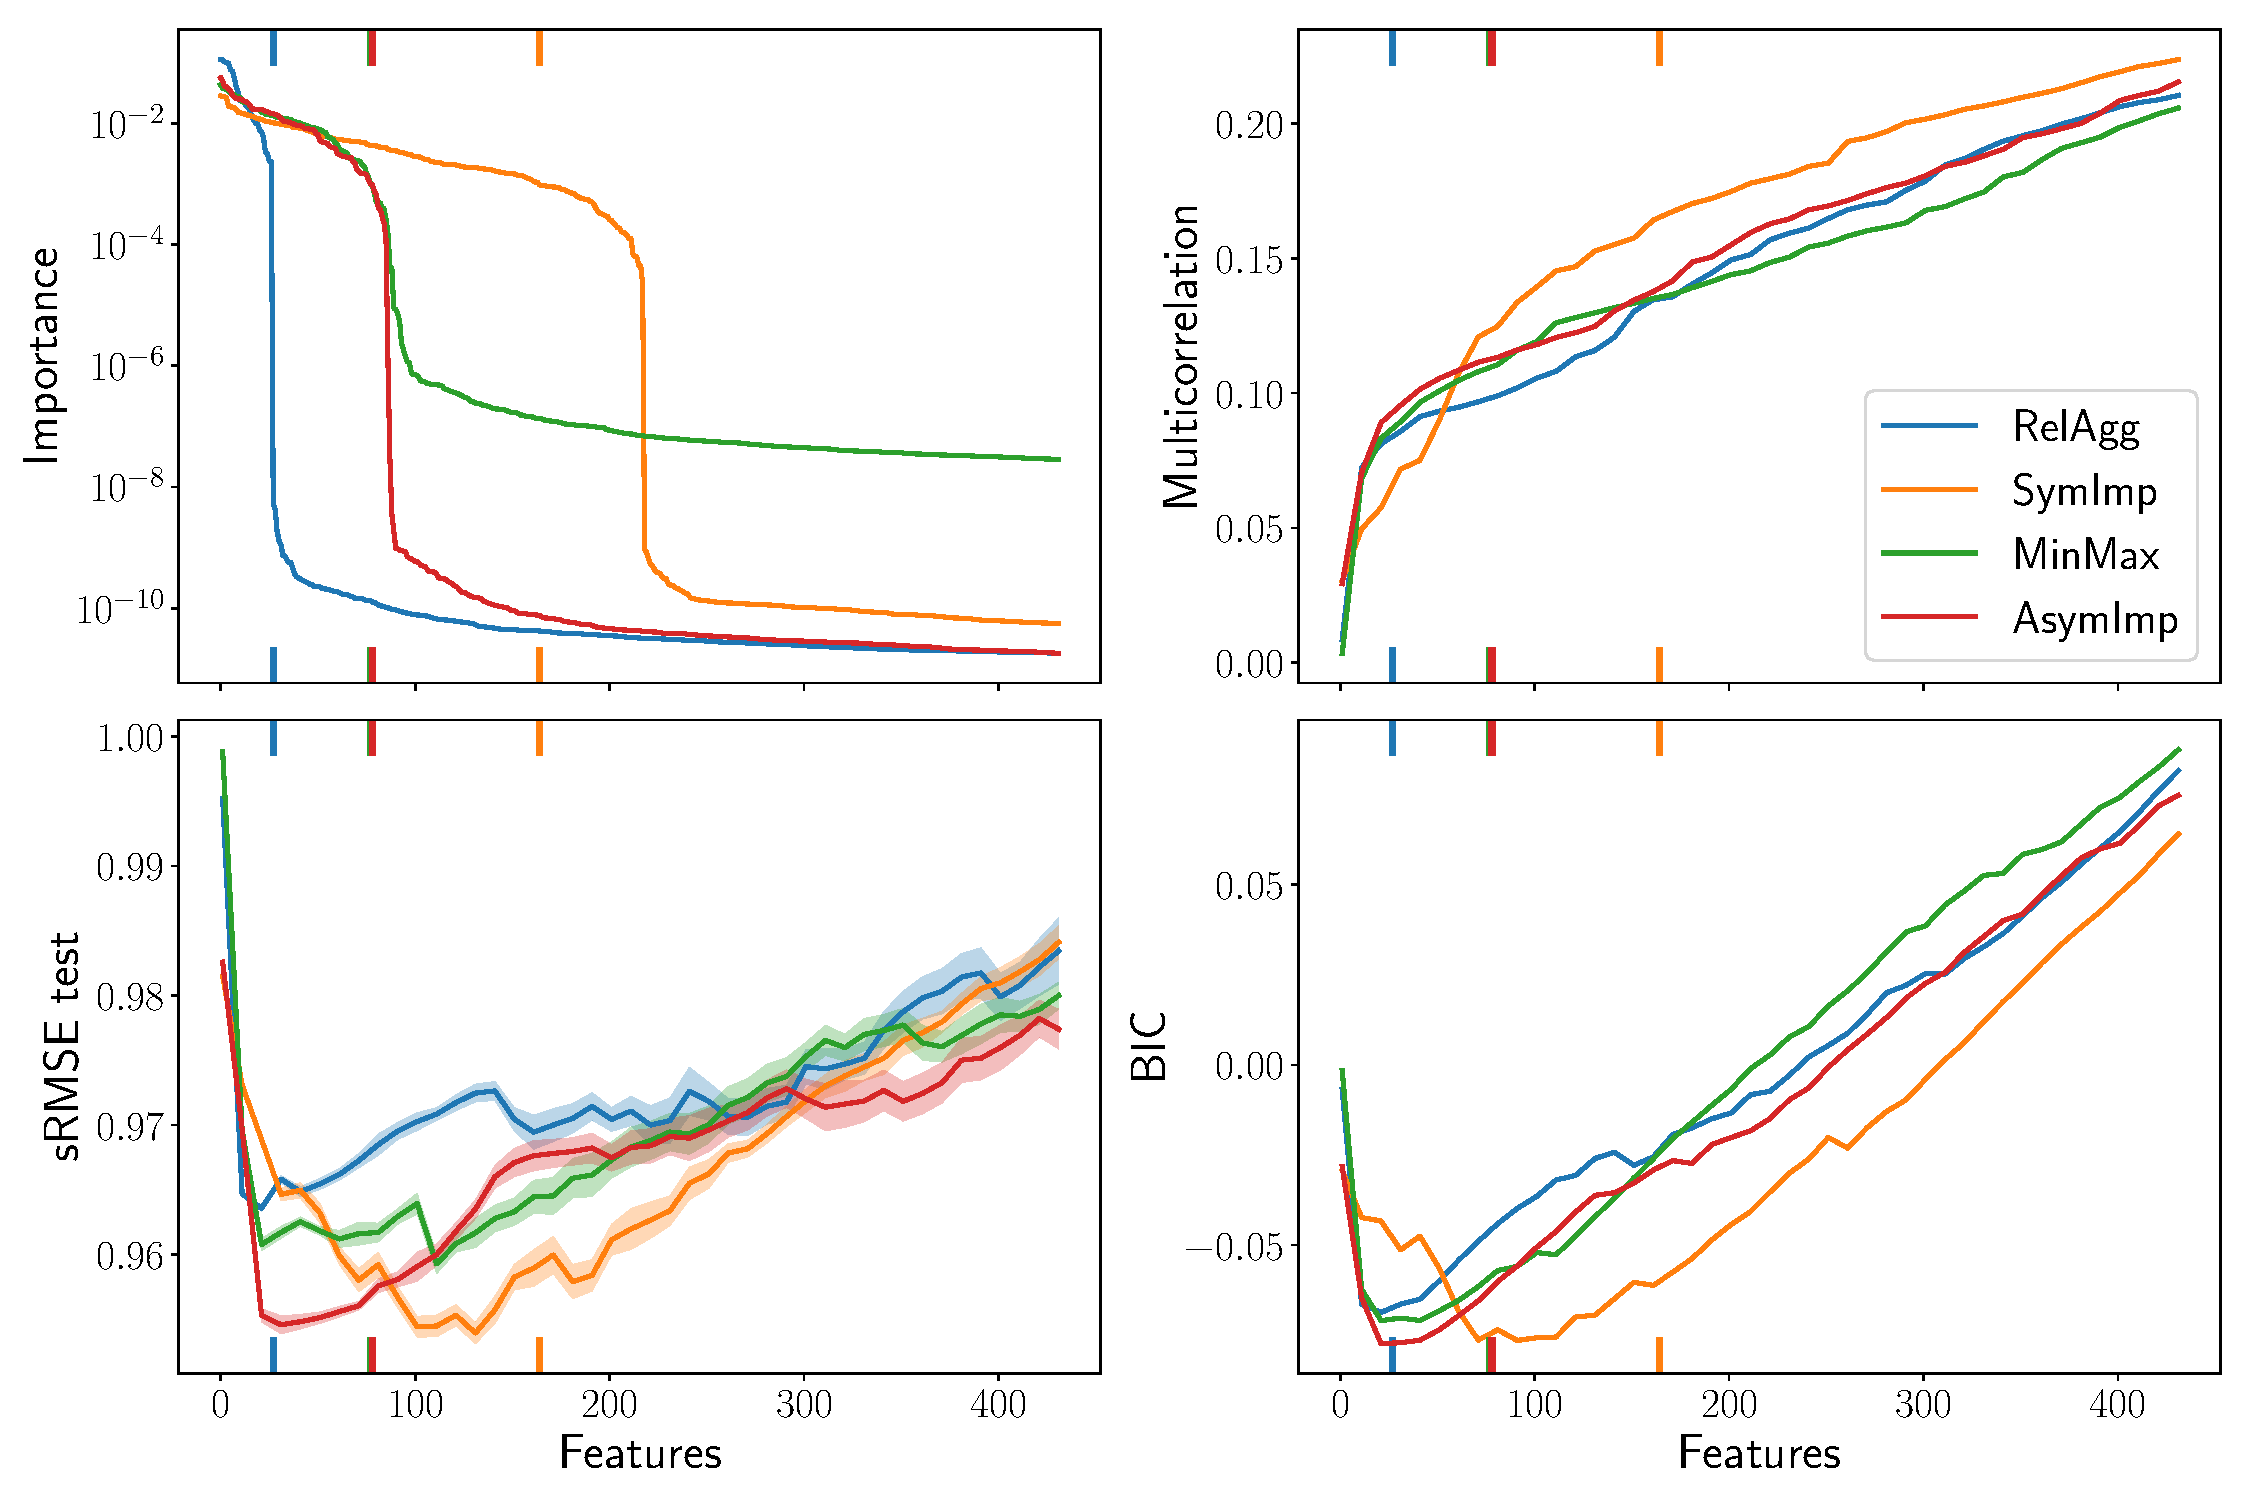
\includegraphics[width=\linewidth]{figs/ecog_3_30_metrics.pdf}
	\caption{Feature selection algorithms evaluation for the ECoG data and the prediction of $k = 30$ timestamps}
	\label{fig:ecog_3_30_metrics}
\end{figure}

To compare the structure of the selected feature subsets and investigate the stability of the selection procedure, we use the bootstrap approach. 
First, the bootstrap data are generated. 
Then, we solve the feature selection problem for each pair of the design and target matrices.
The obtained feature importances are compared. 
We calculate the average pairwise Spearman correlation coefficient and the $\ell_2$ distance as the measures of the algorithms stability.
Table~\ref{tbl:stability} shows the average error, the size of the subset and the described statistics for each method. The error was calculated by fitting the linear model using the $50$ features with the largest importances.
AsymImp gives the least error on the test data. 
The size of the selected feature subsets is overestimated using the threshold $\tau=10^{-4}$. 
The value of~$\tau$ could be cross-validated to get the optimal threshold and feature subset size. 

\begin{table}[]
	\caption{The stability of the selected feature subset}
	\centering
	\begin{tabular}{l|ccccc}
		\hline
		& sRMSE  & $\|\ba\|_0$ & Spearman $\rho$ & $\ell_2$ dist \\ \hline
		RelAgg & 0.965 $\pm$ 0.002 & 26.8 $\pm$ 3.8 & 0.915 $\pm$ 0.016 & 0.145 $\pm$ 0.018   \\
		SymImp & 0.961 $\pm$ 0.001 & 224.4 $\pm$ 9.0 & 0.910 $\pm$ 0.017 & 0.025 $\pm$ 0.002   \\
		MinMax & 0.961 $\pm$ 0.002 & 101.0 $\pm$ 2.1& 0.932 $\pm$ 0.009 & 0.059 $\pm$ 0.004   \\
		AsymImp & 0.955 $\pm$ 0.001 & 85.8 $\pm$ 10.2& 0.926 $\pm$ 0.011 & 0.078 $\pm$ 0.007  \\ \hline
	\end{tabular}
	\label{tbl:stability}
\end{table}

We fit the PLS regression model to the data to compare the dimensionality reduction and feature selection. 
Figure~\ref{fig:pls_vs_k} demonstrates the scaled RMSE on the train and test data with respect to the dimensionality of the latent space~$l$.
The test error reaches its minimum at $l = 11$.
The PLS regression is a more flexible approach compared to the linear model built on the subset of features.
It results in the smallest error, but the model is not sparse.

Figure~\ref{fig:models} compares 3 models: the linear regression and the PLS regression built on 100 features given QPFS and the PLS regression with all features.
We do not include the linear regression with all features because its results are close to the constant prediction. It also provides the result for the Lasso and Elastic Net algorithms that are widely used for feature selection.
We use the AsymImp strategy for QPFS in this experiment.
The number of PLS latent dimension is $l = 15$.
Here, the PLS regression is significantly better than the linear regression with the QPFS features.
It means that the latter model is not flexible enough.
However, the best result is by the PLS regression model combined with the QPFS features. 
This model is sparse since it uses only 100 QPFS features.
The ability of the PLS model to find the optimal latent data representation improves the model performance. 

\begin{figure}[h]
	\begin{minipage}{.41\linewidth}
		\centering
		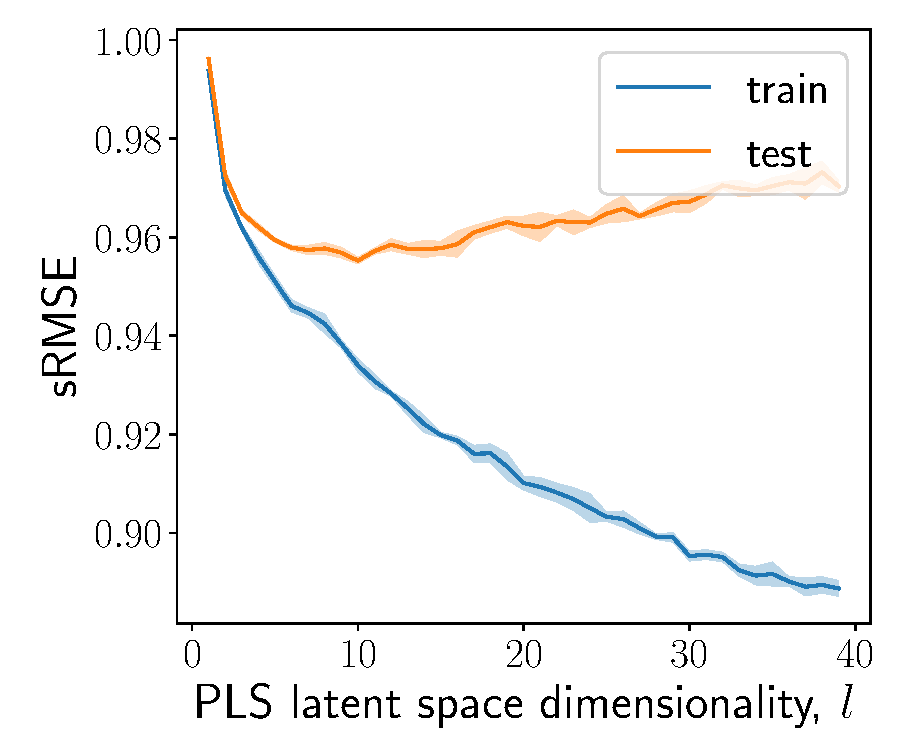
\includegraphics[width=1.\linewidth]{figs/pls_vs_k}
		\caption{Test scaled RMSE for PLS regression models}
		\label{fig:pls_vs_k}
	\end{minipage}%
	\begin{minipage}{.57\linewidth}
		\centering
		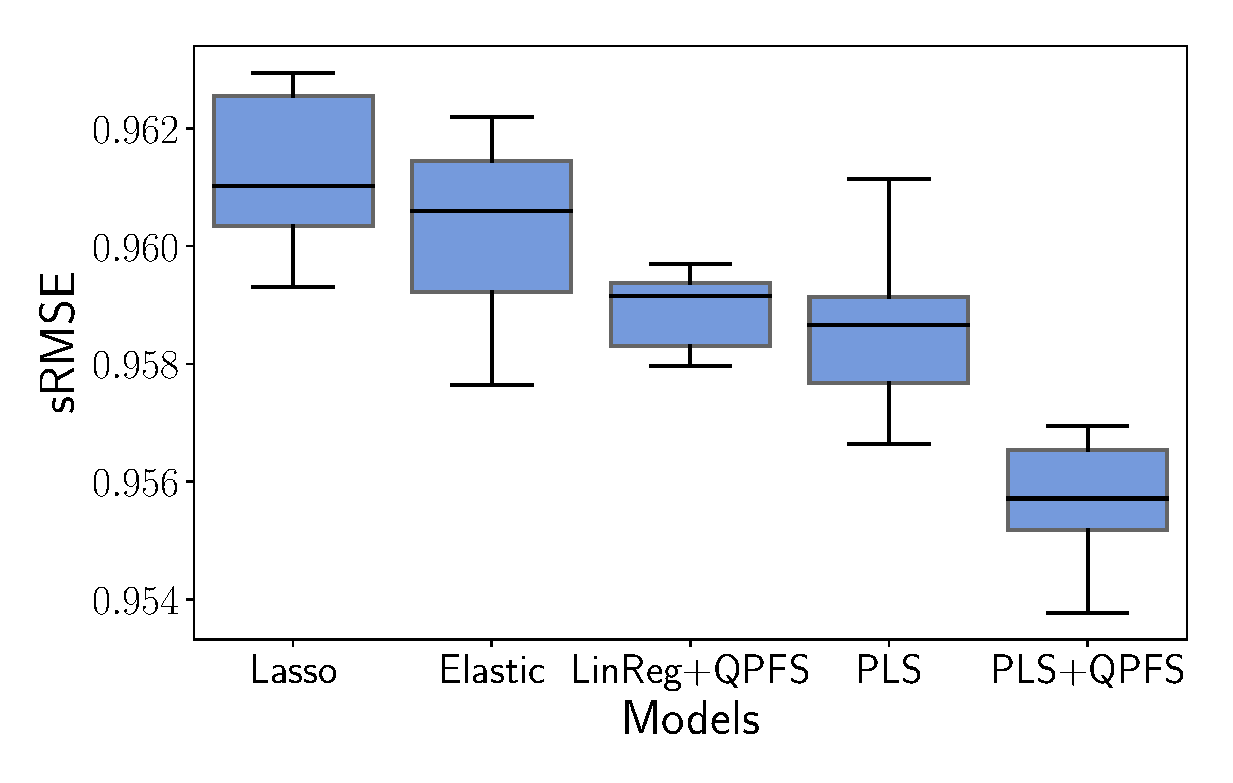
\includegraphics[width=1.\linewidth]{figs/models2}
		\caption{sRMSE box plots for different models}
		\label{fig:models}
	\end{minipage}
\end{figure}

\section{Conclusion}
The study investigates the problem of signal decoding in which the data are highly redundant.
To build a stable, adequate model, we reduced the dimensionality of the problem using the dependencies in both the input and target spaces.
The PLS regression is considered as a linear model for dimensionality reduction.
The quadratic programming approach is investigated as a feature selection algorithm.
The algorithm solves feature selection in a single quadratic programming optimization problem.
The multivariate extensions for the QPFS algorithms are proposed.
The resulting feature subset includes noncorrelated features that are relevant to the most difficult targets.

The computational experiments were carried out using the ECoG data. 
The resulting model predicts the limb position of an exoskeleton using brain signals.
The proposed algorithms outperform the baseline algorithm and reduce the problem dimension significantly.
The combination of feature selection for sparsifying the model and the dimensionality reduction for increasing the model stability give the best result.



\section*{References}
\bibliographystyle{elsarticle-num}
\bibliography{papers_qpfs}
\end{document}
